\section{TCP被动打开-服务器}
        \subsection{基本流程}
            tcp想要被动打开,就必须得先进行listen调用\textbf{(什么时候被调用呢?)}。经过listen调用之后,系统内部其实创建了一个监听套接字,专门负责监听是否有数据发来,而不会负责传输数据。

            当客户端的第一个syn包到达服务器时,其实linux 内核并不会创建sock结构体,而是创建一个轻量级的request\_sock 结构体,里面能唯一确定某个客户端发来的syn的信息,接着就发送syn、ack给客户端。

            客户端一般就接着回ack。这时,我们能从ack中,取出信息,在一堆request\_sock匹配,看看是否之前有这个ack对应的syn发过来过。如果之前发过syn,那么现在我们就能找到request\_sock,也就是客户端syn时建立的request\_sock。 此时,我们内核才会为这条流创建sock结构体,毕竟,sock结构体比request\_sock大的多,犯不着三次握手都没建立起来我就建立一个大的结构体。当三次握手建立以后,内核就建立一个相对完整的sock,所谓相对完整,其实也是不完整。因为如果你写过socket程序你就知道,所谓的真正完整,是建立socket,而不是sock (socket 结构体中有一个指针sock * sk,显然sock只是socket的一个子集)。那么我们什么时候才会创建完整的socket,或者换句话说,什么时候使得sock 结构体和文件系统关联从而绑定一个fd,用这个fd就可以用来传输数据呢?所谓fd(file descriptor),一般是BSD Socket的用法,用在Unix/Linux 系统上。在Unix/Linux系统下,一个socket句柄,可以看做是一个文件,在socket上收发数据,相当于对一个文件进行读写,所以一个socket句柄,通常也用表示文件句柄的fd来表示。

            如果你有socket编程经验,那么你一定能想到,那就是在accept系统调用时,返回了一个fd,所以说,是你在accept 时,你三次握手完成后建立的sock才绑定了一个 fd。
        \subsection{第一次握手:接受SYN段}
            \subsubsection{正常的首次握手函数调用概览}
                \begin{figure}[htb]        
                    \centering
                    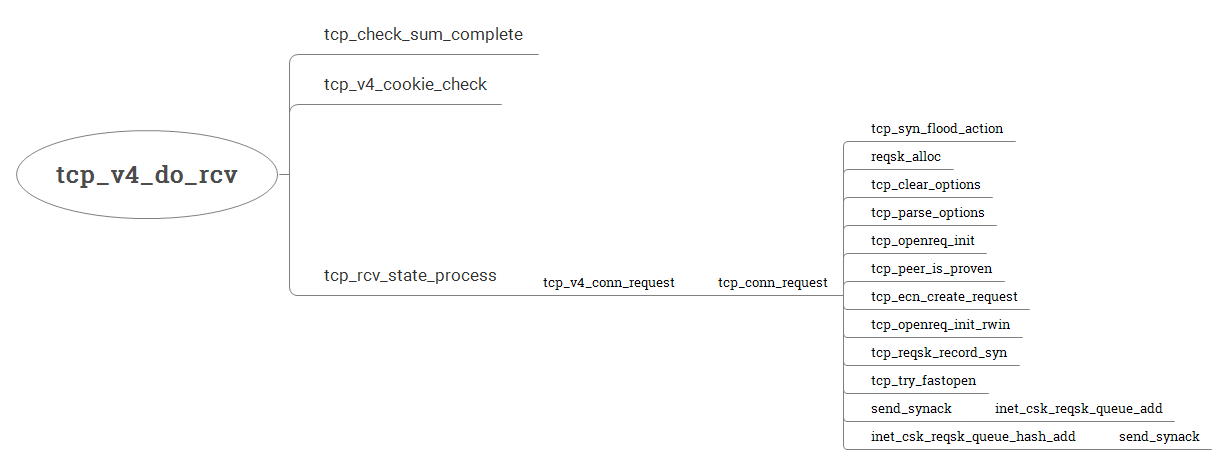
\includegraphics[width=\textwidth]  {images/The First Shake Hand of Server.png}
                \end{figure}       
            \subsubsection{LISTEN状态处理接收到的TCP段}
                在进行第一次握手的时候,TCP一般处于LISTEN状态。传输控制块接收处理的段都由tcp\_v4\_do\_rcv来处理。该函数位于/net/ipv4/tcp\_ipv4.c中。该函数会根据不同的TCP状态进行不同的处理,这里我们只是讨论第一次握手的函数处理过程。
\begin{minted}[linenos]{C}
/* The socket must have it's spinlock held when we get
 * here, unless it is a TCP_LISTEN socket.
 *
 * We have a potential double-lock case here, so even when
 * doing backlog processing we use the BH locking scheme.
 * This is because we cannot sleep with the original spinlock
 * held.
 */
int tcp_v4_do_rcv(struct sock *sk, struct sk_buff *skb)
{
    struct sock *rsk;

    /*省略无关代码*/

    if (tcp_checksum_complete(skb))
        goto csum_err;

    if (sk->sk_state == TCP_LISTEN) {
        struct sock *nsk = tcp_v4_cookie_check(sk, skb);

        if (!nsk)
            goto discard;
        if (nsk != sk) {
            sock_rps_save_rxhash(nsk, skb);
            sk_mark_napi_id(nsk, skb);
            if (tcp_child_process(sk, nsk, skb)) {
                rsk = nsk;
                goto reset;
            }
            return 0;
        }
    } else
        sock_rps_save_rxhash(sk, skb);

    if (tcp_rcv_state_process(sk, skb)) {
        rsk = sk;
        goto reset;
    }
    return 0;

reset:
    tcp_v4_send_reset(rsk, skb);
discard:
    kfree_skb(skb);
    /* Be careful here. If this function gets more complicated and
     * gcc suffers from register pressure on the x86, sk (in \%ebx)
     * might be destroyed here. This current version compiles correctly,
     * but you have been warned.
     */
    return 0;

csum_err:
    TCP_INC_STATS_BH(sock_net(sk), TCP_MIB_CSUMERRORS);
    TCP_INC_STATS_BH(sock_net(sk), TCP_MIB_INERRS);
    goto discard;
}
\end{minted}

                \textbf{函数的参数的意思。表格显示(函数头,函数功能,函数参数及相关简单解释),代码行数放在前面。}
                首先,程序先基于伪首部累加和进行全包的校验和,判断包是否传输正确。

                其次,程序会进行相应的cookie检查。

                最后,程序会继续调用tcp\_rcv\_state\_process函数处理接收到的SYN段。
            
    \subsubsection{LISTEN状态处理请求--tcp\_v4\_cookie\_check}
                该函数如下:
\begin{minted}[linenos]{C}
static struct sock *tcp_v4_cookie_check(struct sock *sk, struct sk_buff *skb)
{
#ifdef CONFIG_SYN_COOKIES
    const struct tcphdr *th = tcp_hdr(skb);

    if (!th->syn)
        sk = cookie_v4_check(sk, skb);
#endif
    return sk;
}
\end{minted}

                可以看出如果系统定义了CONFIG\_SYN\_COOKIES宏的话,并且当前并不是syn包,内核就会继续进行cookie\_v4\_check,否则返回sk。显然对于第一次握手的时候,接收到的确实是syn包,故而不会进行检查。而是直接返回了sk。对于cookie\_v4\_check函数,当内存不足时,就返回NULL,否则就返回sk。
            \subsubsection{LISTEN状态处理SYN段--tcp\_rcv\_state\_process}
                该函数位于/net/ipv4/tcp\_input.c中。函数的简要介绍如下:

                与第一次握手相关的代码如下:

\begin{minted}[linenos]{C}
/*
 *  This function implements the receiving procedure of RFC 793 for
 *  all states except ESTABLISHED and TIME_WAIT.
 *  It's called from both tcp_v4_rcv and tcp_v6_rcv and should be
 *  address independent.
 */

int tcp_rcv_state_process(struct sock *sk, struct sk_buff *skb)
{
    struct tcp_sock *tp = tcp_sk(sk);
    struct inet_connection_sock *icsk = inet_csk(sk);
    const struct tcphdr *th = tcp_hdr(skb);
    struct request_sock *req;
    int queued = 0;
    bool acceptable;

    tp->rx_opt.saw_tstamp = 0;

    switch (sk->sk_state) {
    /*省略无关代码*/

    case TCP_LISTEN:
        if (th->ack)
            return 1;

        if (th->rst)
            goto discard;

        if (th->syn) {
            if (th->fin)
                goto discard;
            if (icsk->icsk_af_ops->conn_request(sk, skb) < 0)
                return 1;

            /* Now we have several options: In theory there is
             * nothing else in the frame. KA9Q has an option to
             * send data with the syn, BSD accepts data with the
             * syn up to the [to be] advertised window and
             * Solaris 2.1 gives you a protocol error. For now
             * we just ignore it, that fits the spec precisely
             * and avoids incompatibilities. It would be nice in
             * future to drop through and process the data.
             *
             * Now that TTCP is starting to be used we ought to
             * queue this data.
             * But, this leaves one open to an easy denial of
             * service attack, and SYN cookies can't defend
             * against this problem. So, we drop the data
             * in the interest of security over speed unless
             * it's still in use.
             */
            kfree_skb(skb);
            return 0;
        }
        goto discard;

        /*省略无关代码*/
discard:
        __kfree_skb(skb);
    }
    return 0;
}
\end{minted}

                显然,所接收到的包的ack、rst、fin字段都不为1,故而执行??行程序。这时开始进行连接检查,判断是否可以允许连接。\textbf{经过不断查找},我们可以发现最终会掉用tcp\_v4\_conn\_request进行处理。如果syn段合法,内核就会为该连接请求创建连接请求块,并且保存相应的信息。否则,就会返回1,原函数会发送reset给客户端表明连接请求失败。

                当然,如果收到的包的ack字段为1,那么由于此时链接还未建立,故该包无效,返回1,并且调用该函数的函数会发送reset包给对方。如果收到的是rst字段或者既有fin又有syn的字段,那就直接销毁,并且释放内存。
            \subsubsection{连接请求处理--tcp\_v4\_conn\_request  tcp\_conn\_request}
                该函数位于/net/ipv4/tcp\_ipv4/tcp\_ipv4.c中,该函数如下:
\begin{minted}[linenos]{C}
int tcp_v4_conn_request(struct sock *sk, struct sk_buff *skb)
{
    /* Never answer to SYNs send to broadcast or multicast */
    if (skb_rtable(skb)->rt_flags & (RTCF_BROADCAST | RTCF_MULTICAST))
        goto drop;

    return tcp_conn_request(&tcp_request_sock_ops,
                &tcp_request_sock_ipv4_ops, sk, skb);

drop:
    NET_INC_STATS_BH(sock_net(sk), LINUX_MIB_LISTENDROPS);
    return 0;
}
\end{minted}
                
        首先,如果一个SYN段是要被发送到广播地址和组播地址,则直接drop掉,然后返回0。否则的话,就继续调用tcp\_conn\_request进行连接处理。
\begin{minted}[linenos]{C}
int tcp_conn_request(struct request_sock_ops *rsk_ops,
             const struct tcp_request_sock_ops *af_ops,
             struct sock *sk, struct sk_buff *skb)
{
    struct tcp_fastopen_cookie foc = { .len = -1 };
    __u32 isn = TCP_SKB_CB(skb)->tcp_tw_isn;
    struct tcp_options_received tmp_opt;
    struct tcp_sock *tp = tcp_sk(sk);
    struct sock *fastopen_sk = NULL;
    struct dst_entry *dst = NULL;
    struct request_sock *req;
    bool want_cookie = false;
    struct flowi fl;

    /* TW buckets are converted to open requests without
     * limitations, they conserve resources and peer is
     * evidently real one.
     */
    if ((sysctl_tcp_syncookies == 2 ||
         inet_csk_reqsk_queue_is_full(sk)) && !isn) {
        want_cookie = tcp_syn_flood_action(sk, skb, rsk_ops->slab_name);
        if (!want_cookie)
            goto drop;
    }
\end{minted}
                首先,前面???如果SYN请求队列已满并且isn为0,然后通过函数\textbf{tcp\_syn\_flood\_action}判断是否需要发送syncookie。如果没有启用syncookie的话,就会返回false,此时不能接收新的SYN请求,会将所收到的包丢掉。
\begin{minted}[linenos]{C}
    /* Accept backlog is full. If we have already queued enough
     * of warm entries in syn queue, drop request. It is better than
     * clogging syn queue with openreqs with exponentially increasing
     * timeout.
     */
    if (sk_acceptq_is_full(sk) && inet_csk_reqsk_queue_young(sk) > 1) {
        NET_INC_STATS_BH(sock_net(sk), LINUX_MIB_LISTENOVERFLOWS);
        goto drop;
    }
\end{minted}

        \textbf{warm entries}               
        
        如果连接队列长度已经达到上限且SYN请求队列中至少有一个握手过程中没有重传过段,则丢弃当前请求。

\begin{minted}[linenos]{C}
    req = inet_reqsk_alloc(rsk_ops, sk, !want_cookie);
    if (!req)
        goto drop;
\end{minted}
            
        这时调用reqsk\_alloc()分配一个连接请求块,用于保存连接请求信息,同时初始化在连接过程中用来发送ACK/RST段的操作集合,以便在建立连接过程中能方便地调用这些接口。

\begin{minted}[linenos]{C}
    tcp_rsk(req)->af_specific = af_ops;
\end{minted}

        这一步进行的是为了保护BGP会话。???
        
\begin{minted}[linenos]{C}
    tcp_rsk(req)->af_specific = af_ops;

    tcp_clear_options(&tmp_opt);
    tmp_opt.mss_clamp = af_ops->mss_clamp;
    tmp_opt.user_mss  = tp->rx_opt.user_mss;
    tcp_parse_options(skb, &tmp_opt, 0, want_cookie ? NULL : &foc);
\end{minted}

        之后,清除TCP选项后初始化mss\_vlamp和user\_mss.然后调用tcp\_parse\_options解析SYN段中的TCP选项,查看是否有相关的选项。
\begin{minted}[linenos]{C}
    if (want_cookie && !tmp_opt.saw_tstamp)
        tcp_clear_options(&tmp_opt);
\end{minted}

        如果启动了syncookies,并且TCP段中没有存在时间戳(why,the reason?),则清除已经解析的TCP选项。

\begin{minted}[linenos]{C}
    tmp_opt.tstamp_ok = tmp_opt.saw_tstamp;
    tcp_openreq_init(req, &tmp_opt, skb, sk);
\end{minted}

        这时,根据收到的SYN段中的选项和序号来初始化连接请求块信息。

\begin{minted}[linenos]{C}
    /* Note: tcp_v6_init_req() might override ir_iif for link locals */
    inet_rsk(req)->ir_iif = sk->sk_bound_dev_if;

    af_ops->init_req(req, sk, skb);

    if (security_inet_conn_request(sk, skb, req))
        goto drop_and_free;
\end{minted}

        这一部分于IPV6以及安全检测有关,这里不进行详细讲解。安全检测失败的话,就会丢弃SYN段。

\begin{minted}[linenos]{C}
    if (!want_cookie && !isn) {
        /* VJ's idea. We save last timestamp seen
         * from the destination in peer table, when entering
         * state TIME-WAIT, and check against it before
         * accepting new connection request.
         *
         * If "isn" is not zero, this request hit alive
         * timewait bucket, so that all the necessary checks
         * are made in the function processing timewait state.
         */
        if (tcp_death_row.sysctl_tw_recycle) {
            bool strict;

            dst = af_ops->route_req(sk, &fl, req, &strict);

            if (dst && strict &&
                !tcp_peer_is_proven(req, dst, true,
                        tmp_opt.saw_tstamp)) {
                NET_INC_STATS_BH(sock_net(sk), LINUX_MIB_PAWSPASSIVEREJECTED);
                goto drop_and_release;
            }
        }
        /* Kill the following clause, if you dislike this way. */
        else if (!sysctl_tcp_syncookies &&
             (sysctl_max_syn_backlog - inet_csk_reqsk_queue_len(sk) <
              (sysctl_max_syn_backlog >> 2)) &&
             !tcp_peer_is_proven(req, dst, false,
                         tmp_opt.saw_tstamp)) {
            /* Without syncookies last quarter of
             * backlog is filled with destinations,
             * proven to be alive.
             * It means that we continue to communicate
             * to destinations, already remembered
             * to the moment of synflood.
             */
            pr_drop_req(req, ntohs(tcp_hdr(skb)->source),
                    rsk_ops->family);
            goto drop_and_release;
        }

        isn = af_ops->init_seq(skb);
    }
\end{minted}

        如果没有开启syncookie并且isn为0的话,在距中的第一个if从对段信息块中获取时间戳,在新的连接请求之前检测\textbf{PAWS}。后边的表明在没有启动syncookies的情况下受到synflood攻击,丢弃收到的段。之后由源地址,源端口,目的地址以及目的端口计算出服务端初始序列号。

\begin{minted}[linenos]{C}
    if (!dst) {
        dst = af_ops->route_req(sk, &fl, req, NULL);
        if (!dst)
            goto drop_and_free;
    }

    tcp_ecn_create_request(req, skb, sk, dst);

    if (want_cookie) {
        isn = cookie_init_sequence(af_ops, sk, skb, &req->mss);
        req->cookie_ts = tmp_opt.tstamp_ok;
        if (!tmp_opt.tstamp_ok)
            inet_rsk(req)->ecn_ok = 0;
    }

    tcp_rsk(req)->snt_isn = isn;
    tcp_rsk(req)->txhash = net_tx_rndhash();
    tcp_openreq_init_rwin(req, sk, dst);
    if (!want_cookie) {
        tcp_reqsk_record_syn(sk, req, skb);
        fastopen_sk = tcp_try_fastopen(sk, skb, req, &foc, dst);
    }
    if (fastopen_sk) {
        af_ops->send_synack(fastopen_sk, dst, &fl, req,
                    &foc, false);
        /* Add the child socket directly into the accept queue */
        inet_csk_reqsk_queue_add(sk, req, fastopen_sk);
        sk->sk_data_ready(sk);
        bh_unlock_sock(fastopen_sk);
        sock_put(fastopen_sk);
    } else {
        tcp_rsk(req)->tfo_listener = false;
        if (!want_cookie)
            inet_csk_reqsk_queue_hash_add(sk, req, TCP_TIMEOUT_INIT);
        af_ops->send_synack(sk, dst, &fl, req,
                    &foc, !want_cookie);
        if (want_cookie)
            goto drop_and_free;
    }
    reqsk_put(req);
    return 0;

drop_and_release:
    dst_release(dst);
drop_and_free:
    reqsk_free(req);
drop:
    NET_INC_STATS_BH(sock_net(sk), LINUX_MIB_LISTENDROPS);
    return 0;
\end{minted}

                暂时不懂,,,,等等在分析。。。。。。。

            \subsubsection{inet\_csk\_reqsk\_queue\_add}

\begin{minted}[linenos]{C}
struct sock *inet_csk_reqsk_queue_add(struct sock *sk,
                      struct request_sock *req,
                      struct sock *child)
{
    struct request_sock_queue *queue = &inet_csk(sk)->icsk_accept_queue;

    spin_lock(&queue->rskq_lock);
    if (unlikely(sk->sk_state != TCP_LISTEN)) {
        inet_child_forget(sk, req, child);
        child = NULL;
    } else {
        req->sk = child;
        req->dl_next = NULL;
        if (queue->rskq_accept_head == NULL)
            queue->rskq_accept_head = req;
        else
            queue->rskq_accept_tail->dl_next = req;
        queue->rskq_accept_tail = req;
        sk_acceptq_added(sk);
    }
    spin_unlock(&queue->rskq_lock);
    return child;
}
\end{minted}

                这一个函数所进行的操作就是直接将请求挂在接收队列中。

            \subsubsection{inet\_csk\_reqsk\_queue\_hash\_add}

\begin{minted}[linenos]{C}
void inet_csk_reqsk_queue_hash_add(struct sock *sk, struct request_sock *req,
                   unsigned long timeout)
{
    reqsk_queue_hash_req(req, timeout);
    inet_csk_reqsk_queue_added(sk);
}
\end{minted}

                首先将连接请求块保存到父传输请求块的散列表中,并设置定时器超时时间。之后更新已存在的连接请求块数,并启动连接建立定时器。
%----------------------------------------------------------------------------------------
%                   Server:     Send    SYN+ACK
%----------------------------------------------------------------------------------------

        \subsection{第二次握手:发送SYN+ACK段}
            在第一次握手的最后调用了af\_ops->send\_synack函数,而该函数最终会调用tcp\_v4\_send\_synack函数进行发送,故而这里我们这里就从这个函数进行分析。
            \subsubsection{函数调用关系}            
                第二次握手的调用函数关系图如下:
                %\begin{figure}[htb]        
                %   \center{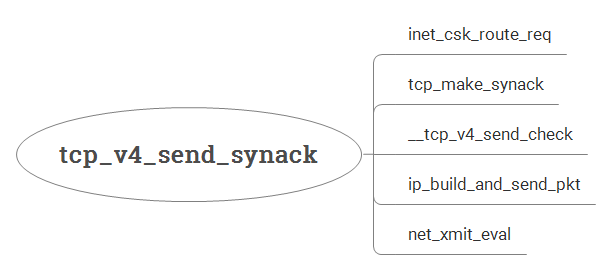
\includegraphics[width=\textwidth]  {The Second Shake Hand of Server.png}}
                %\end{figure}   
            \subsubsection{tcp\_v4\_send\_synack}
\begin{minted}[linenos]{C}
/*
 *  Send a SYN-ACK after having received a SYN.
 *  This still operates on a request_sock only, not on a big
 *  socket.
 */
static int tcp_v4_send_synack(const struct sock *sk, struct dst_entry *dst,
                  struct flowi *fl,
                  struct request_sock *req,
                  struct tcp_fastopen_cookie *foc,
                  bool attach_req)
{
    const struct inet_request_sock *ireq = inet_rsk(req);
    struct flowi4 fl4;
    int err = -1;
    struct sk_buff *skb;

    /* First, grab a route. */
    if (!dst && (dst = inet_csk_route_req(sk, &fl4, req)) == NULL)
        return -1;

    skb = tcp_make_synack(sk, dst, req, foc, attach_req);

    if (skb) {
        __tcp_v4_send_check(skb, ireq->ir_loc_addr, ireq->ir_rmt_addr);

        err = ip_build_and_send_pkt(skb, sk, ireq->ir_loc_addr,
                        ireq->ir_rmt_addr,
                        ireq->opt);
        err = net_xmit_eval(err);
    }

    return err;
}
\end{minted}                
                首先,如果传进来的dst为空或者根据连接请求块中的信息查询路由表,如果没有查到,那么就直接推出。

                否则就跟据当前的传输控制块,路由信息,请求等信息构建syn+ack段。

                如果构建成功的话,就生成TCP校验码,然后调用ip\_build\_and\_send\_pkt生成IP数据报并且发送出去。

                net\_xmit\_eval是什么,待考虑。
            \subsubsection{tcp\_make\_synack}
                该函数用来构造一个SYN+ACK段,并初始化TCP首部及SKB中的各字段项,填入相应的选项,如MSS,SACK,窗口扩大银子,时间戳等。函数如下:
\begin{minted}[linenos]{C}
/**
 * tcp_make_synack - Prepare a SYN-ACK.
 * sk: listener socket
 * dst: dst entry attached to the SYNACK
 * req: request_sock pointer
 *
 * Allocate one skb and build a SYNACK packet.
 * @dst is consumed : Caller should not use it again.
 */
struct sk_buff *tcp_make_synack(const struct sock *sk, struct dst_entry *dst,
                struct request_sock *req,
                struct tcp_fastopen_cookie *foc,
                bool attach_req)
{
    struct inet_request_sock *ireq = inet_rsk(req);
    const struct tcp_sock *tp = tcp_sk(sk);
    struct tcp_md5sig_key *md5 = NULL;
    struct tcp_out_options opts;
    struct sk_buff *skb;
    int tcp_header_size;
    struct tcphdr *th;
    u16 user_mss;
    int mss;

    skb = alloc_skb(MAX_TCP_HEADER, GFP_ATOMIC);
    if (unlikely(!skb)) {
        dst_release(dst);
        return NULL;
    }
\end{minted}

                首先为将要发送的数据申请发送缓存,\textbf{unlikely函数待分析???},如果没有申请到,那就会返回NULL。
